%------------------------------------------------
%
% Flow.tex 
%
% This section introduces the incident management
% process flow.
%------------------------------------------------
\section[Attività di processo]{attività di processo}
\label{em-flow}
Nella seguente sezione viene riportato il flusso delle attività presenti nel processo che gli operatori del \english{Service Desk} devono seguire quando sono generati degli eventi. In Figura \ref{em-flow-img} è visualizzato un diagramma di flusso rappresentante le attività, mentre ogni singolo \english{step} è elencato in Tabella \ref{em-flow-table}.

\begin{figure}[htbp]
\centering
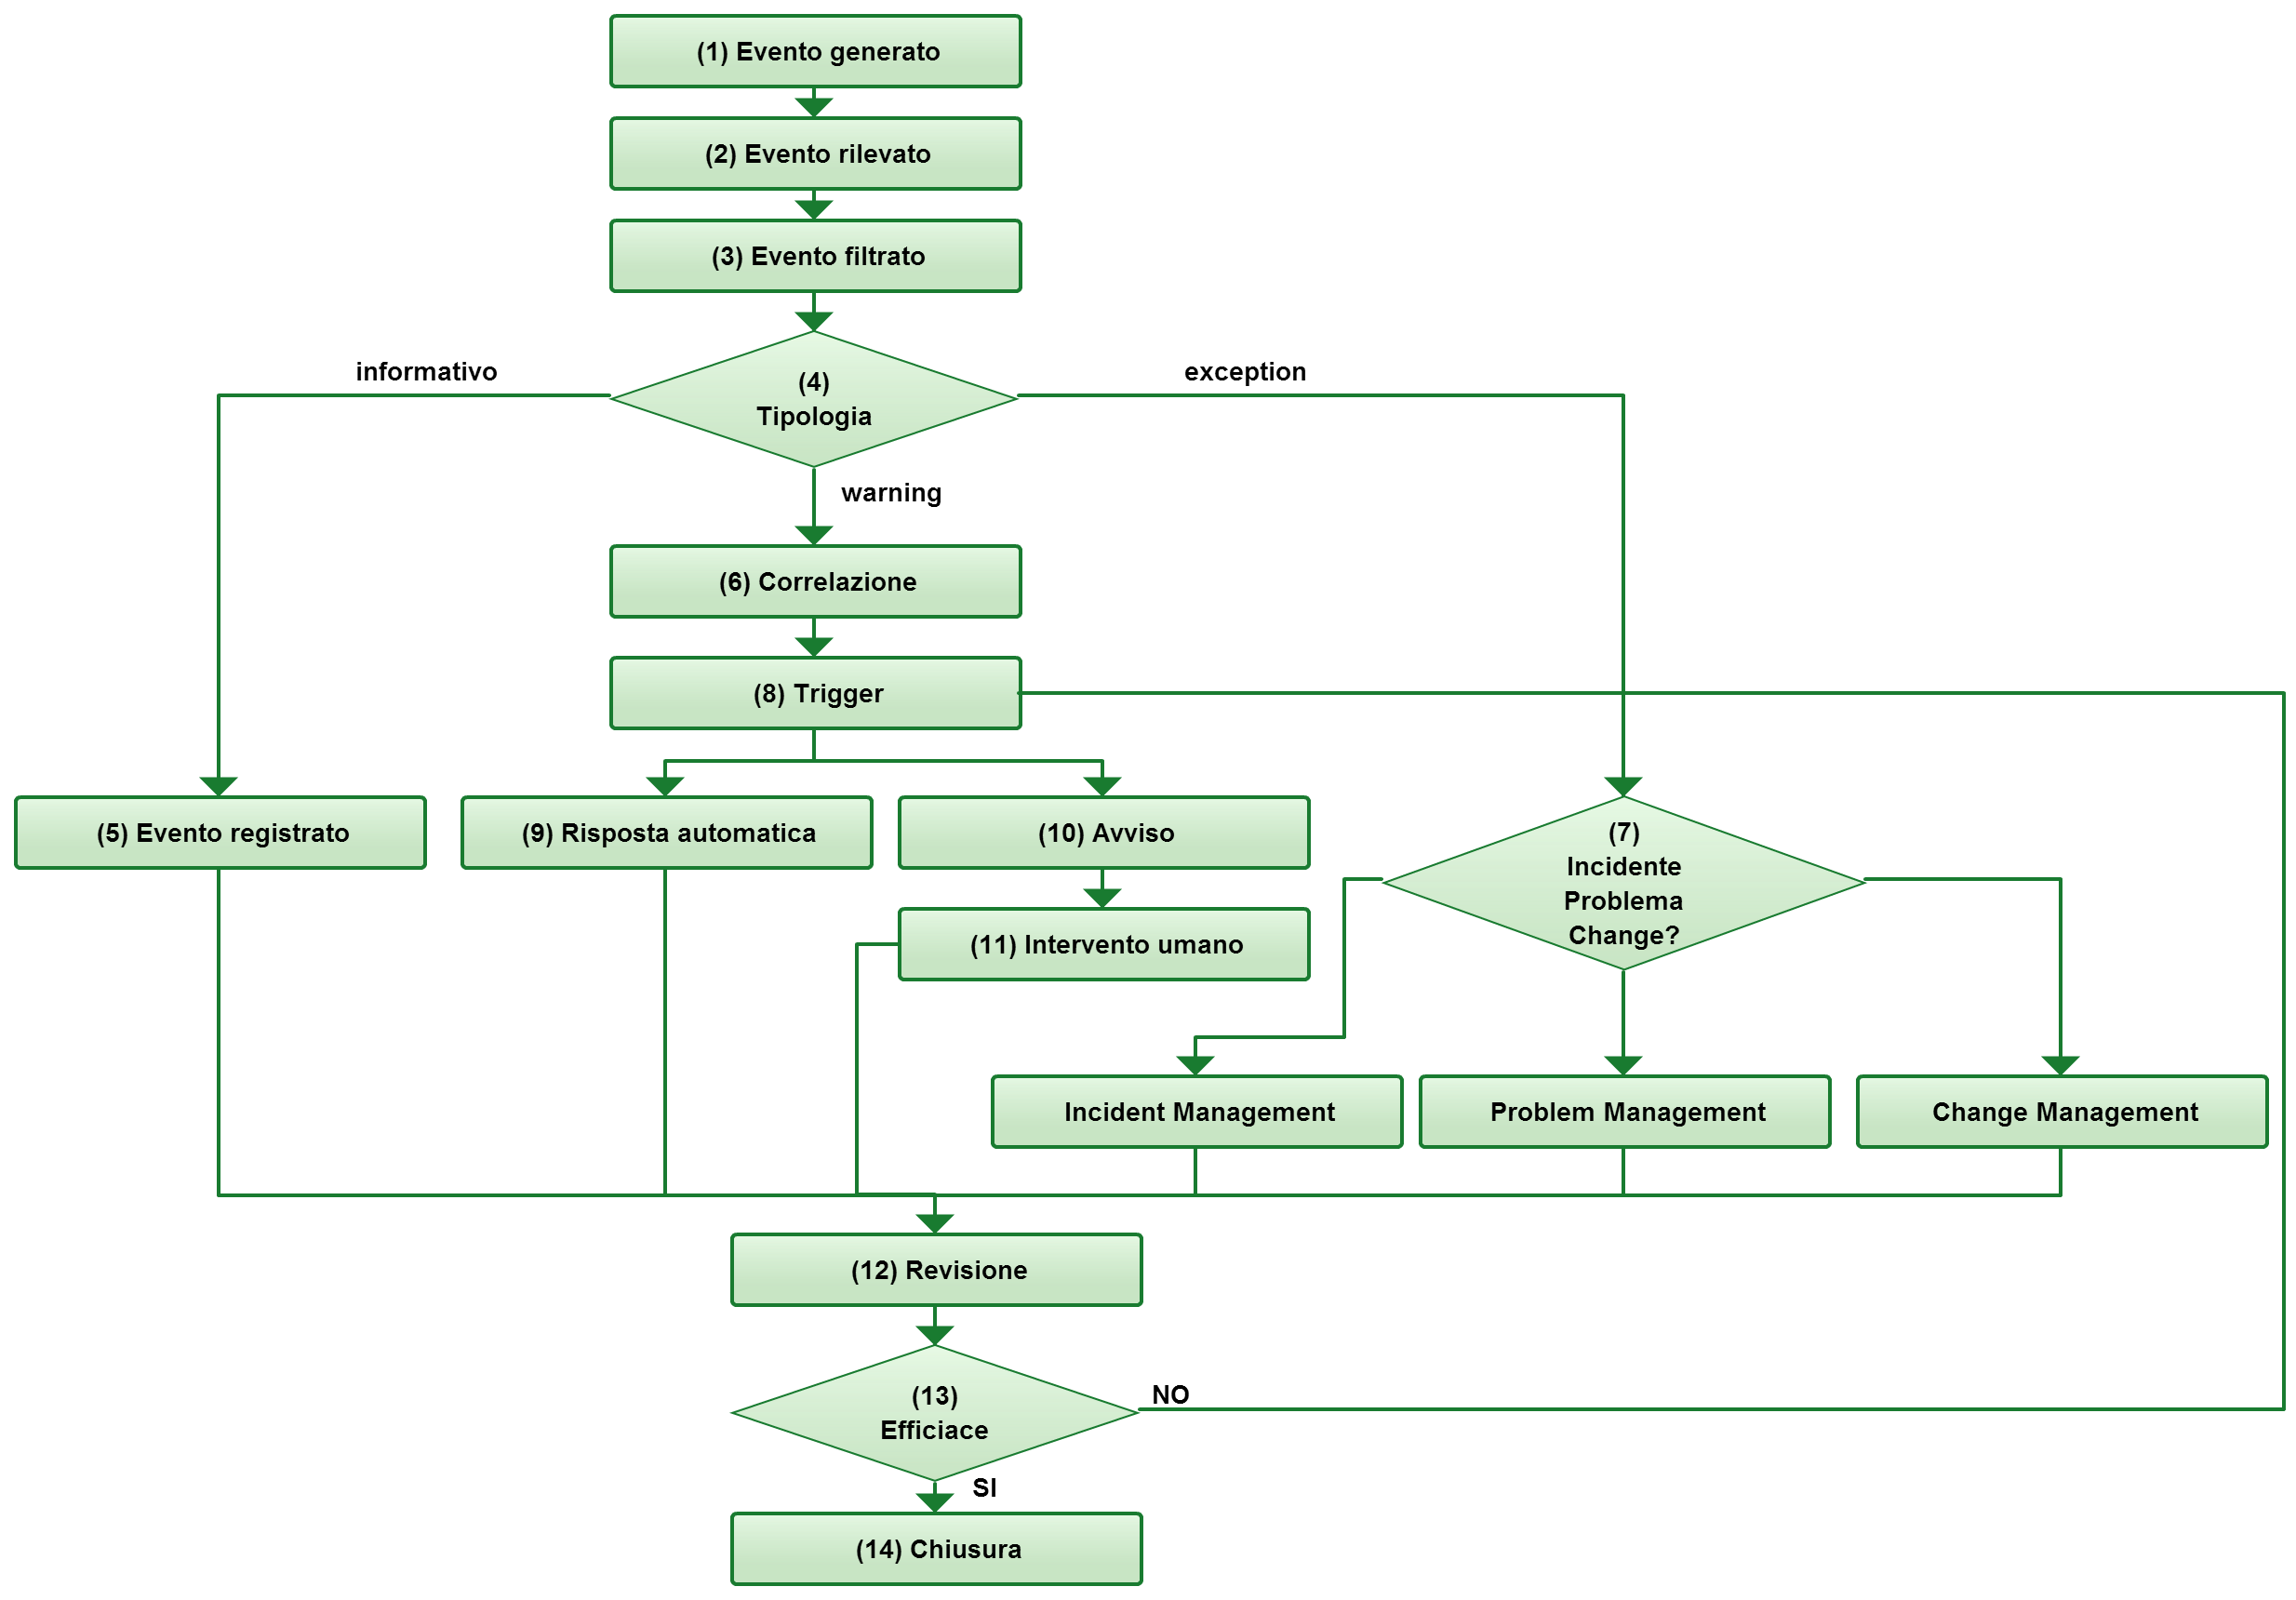
\includegraphics[scale=0.25]{Images/Diagrams/Event_Management.png}
\caption{Flusso attività del processo di \ac{Event-Management}}
\label{em-flow-img}
\end{figure}

\begin{center}
\begin{longtable}{| p{3cm} | p{2cm} | p {7cm} |}
\caption{Elenco attività di processo}
\label{em-flow-table}\\
\hline
\multicolumn{1}{| c |}{\textbf{Ruolo}} & \multicolumn{1}{| c |}{\textbf{Step}} & \multicolumn{1}{| c |}{\textbf{Descrizione}}\\
\hline
\endfirsthead
\hline
\multicolumn{1}{| c |}{\textbf{Ruolo}} & \multicolumn{1}{| c |}{\textbf{Step}} & \multicolumn{1}{| c |}{\textbf{Descrizione}}\\
\hline
\endhead
\multirow{9}{*}{Sistema/Sensore} & 1 & L'evento viene generato dal sistema oppure dal sensore.\\
\cline{2-3}
& 2 & L'evento viene comunicato al \english{tool} di supporto (sistema passivo) oppure il \english{tool} di supporto si accorge che un evento è stato scatenato (sistema attivo).\\
\cline{2-3}
& 3 & L'evento viene filtrato cosi che possa essere categorizzato.\\
\cline{2-3}
& 5 & L'evento generato è di tipo informativo per cui è sufficiente registrarlo nel \english{database} logico.\\
\cline{2-3}
& 6 & L'evento è di tipo \english{warning} e viene ora correlato (ad eventi di tipo \english{warning} simili) dal \english{tool} di supporto che decide quale azione svolgere sulla base dei criteri con cui è stato programmato.\\
\cline{2-3}
& 7 & Il sistema ha generato un evento di tipo \english{exception} ed in base a criteri con cui verrà programmato il \english{tool} di supporto verrà aperto un \english{ticket} verso il processo di \ac{Incident-Management} oppure \ac{Problem-Management} oppure \acs{Change-Management}.\\
\cline{2-3}
& 8 & Un \english{trigger} verifica se l'azione decisa ed applicata dopo la correlazione ha risolto l'evento. Se l'evento è risolto proseguire con lo \english{step} 9 altrimenti con lo \english{step} 10.\\
\cline{2-3}
& 9 & Il \english{trigger} ha verificato che le cause che hanno generato l'evento non sono più presenti.\\
\cline{2-3}
& 10 & Il \english{trigger} ha verificato che l'anomalia non si è risolta attraverso \english{script} automatici ed notifica che è necessario un intervento umano.\\
\hline
\multirow{4}{*}{operatore} & 11 & Il tecnico del \english{Service Desk} interviene per valutare la situazione e decidere l'azione più opportuna da intraprendere.\\
\cline{2-3}
& 12 & Viene eseguita una revisione per valutare se le cause che hanno generato l'evento sono state eliminate.\\
\cline{2-3}
& 13 & Se la revisione ha avuto esito positivo si procede con la chiusura altrimenti si torna nella fase di analisi.\\
\cline{2-3}
& 14 & Vengono memorizzate e tracciate in modo persistente tutte le informazioni sull'intervento e l'evento viene segnalato come concluso.\\
\hline
\end{longtable}
\end{center}